\selectlanguage{french}
\part{Introduction Générale}

\chapter*[Introduction]{}

\vspace{-5cm}

\og L'altération de l'environnement du fait des actions
humaines a déclenché la sixième grande extinction de l'histoire de la vie\ldots\fg
\autocites{stuart-chapin-iii2000a}

Voici comment les experts mondiaux concluent sur le statut actuel et les
évolutions futures de la biodiversité, incluant la diversité de tous les groupes
taxonomiques à tous les niveaux : diversité génétique, diversité spécifique,
diversité des communautés et des écosystèmes dans tous les habitats naturels.
Dans le contexte du changement climatique et du déclin de la biodiversité, il
est particulièrement important d'améliorer notre compréhension de la réponse
des espèces aux changements globaux afin de prédire leur devenir. Afin de faire
face à ce défit, il est d'abord nécessaire de comprendre correctement le
fonctionnement des écosystèmes et des populations qui les habites et de leur
dynamique. 

Le travail présenté dans cette thèse s'inscrit dans le champs de l'étude
expérimentale et théorique de la dynamique des populations. Plus précisément, ce
travail apporte des éléments réponses quant aux mécanismes fins de régulation
des populations, via la densité dépendance, notamment lorsque l'on considère
leur structure en taille.
Nous me suis d'abord intéressé à la description de dynamiques
de populations structurées en taille et des mécanismes en jeu dans leur
régulation. Ceci nous a conduit à identifier la compétition par interférence
comme un élément clé dans la régulation des populations.
Nous avons ensuite établi un cadre théorique au rôle de l'interférence dans la
dynamique des populations. Puis, en intervenant expérimentalement sur la 
structure en taille de populations, nous avons pu démontrer 
l'existence de certains mécanismes proposés à la suite des études descriptive et
théorique.
Enfin, nous nous sommes intéressés au rôle de la température sur la dynamique
des populations structurées, et à ses interactions avec les mécanismes de densité
dépendance.


\chapter{État de l'art}

\section{Les conséquences écologiques de la structuration des populations}

\lettrine[lines=3]{P}{our comprendre} le fonctionnement des écosystèmes et les
réponses des espèces à leur environnement, il est d'important de comprendre leur démographie et la
dynamique de leur populations. De nombreuses études empiriques ont montré que
ces populations étaient structurées de façon non triviales. C'est un 
résultat très général qui a été vérifié à de nombreuses reprises, que ce soit en
laboratoire, comme chez la drosophile ou chez des acariens par exemple, ou dans
des populations naturelles telles que les populations de moutons de Soay ou de cerfs
élaphe. 
Cela implique que la description d'une population comme un tout ou comme
un assemblage de classe crées artificiellement représente généralement mal la
réalité et n'intègre pas suffisamment de complexité pour décrire fidèlement les
mécanismes qui régulent sa dynamique.

\subsection{Différents niveaux de structuration}

Dans une population, la structure émerge de l'hétérogénéité entre les
individus d'une même espèce. Plusieurs formes de structures ont été
classiquement prises en compte en écologie.

\subsubsection{Structuration spatiale}

Une première forme de structuration évidente est la structuration spatiale. Ceci
décrit comment les individus d'une population s'organisent dans l'espace, et ce
faisant, modifient leurs interactions entre eux et avec leur environnement. 

La structuration spatiale des populations répond souvent à l'hétérogénéité de
leur habitat. Ces hétérogénéités ont des conséquences directes sur la dynamiques
des populations, par exemple en modifiant les schémas de dispersion des
individus \autocite{hiebeler2000a}, leur fitness \autocite{zajkac2008a},
l'accès aux ressources \autocite{burger2008a}, la sensibilité aux parasite ou
pathogènes \autocite{su2009a}, \textit{etc}.

L'étude de la dynamique des populations structurées spatialement constitue un
champs de recherche extrêmement large et varié auquel notre étude ne se rattache
pas directement. 

\subsubsection{Structuration génétique}

Conséquence de la structuration spatiale, les population sont souvent également
structurées génétiquement. Les individus les plus proches les uns des autres,
notamment dans des méta-populations, sont également plus proches génétiquement
que des individus spatialement éloignés. L'analyse génétique d'une population
permet alors d'obtenir des informations sur ses origines et sa structuration
spatiale \autocite{repaci2006a,booth2009a,jorde2007a}.

\subsubsection{Structuration en stades}
\subsubsection{Structuration en âges}
\subsubsection{Structuration physiologique}

\subsection{Importance de la taille corporelle}

\subsubsection{Sur les traits d'histoire de vie}

\subsubsection{Sur la structure et la dynamique des populations}

\subsubsection{Sur la structure et la dynamique des communautés}





% Une des causes principales de cette hétérogénéité
% vient du cycle de vie de l'espèce et des différentes étapes qu'un individu
% traverse au cours de ce cycle. 

\section{Mécanismes de densité dépendance}

\section{Le rôle de la température}

\section{Problématiques}	


\chapter{Éléments de méthodologie}

Le travail présenté dans cette thèse repose sur de travaux expérimentaux et
théoriques. En particulier, la partie expérimentale a été centrée sur l'étude de
populations de Collemboles de l'espèce \textit{Folsomia candida} élevée en
microcosmes au laboratoire. Dans ce chapitre, nous présenterons notre espèce
modèle du point de vu de sa biologie, de son intérêt pour les études menées, et
des conditions d'élevages. Puis nous détaillerons quelques développements
méthodologique qui ont permis l'accomplissement de nos travaux. 

\section{Le collembole, un modèle d'étude en écologie des populations}
\sectionmark{Le collembole modèle d'étude}

\subsection{Quelques généralités}

les Collemboles sont de petits arthropodes hexapodes entognathes aptères
mesurant généralement 1 à 5 mm. C'est un groupe très anciens qui compte
notamment l'un des plus vieux fossiles d'héxapode connu (\textit{Rhyniella
praecursor}). Aujourd'hui, plus de 8000 espèces ont été décrites
\autocites{bellinger2014a}, réparties dans l'ensemble des écosystèmes connus, en
faisant une des lignées d'arthropodes les plus communes au monde. Bien que
proches des Insectes, les Collemboles forment une classe à part, à côté des
Diploures, des Protoures et des Insectes \autocites{grimaldi2010a}. Ils sont
classés en quatre ordres: les Poduromorphes, les Entomobryomorphes, les
Symphypléones et les Néanuridés.

Les Collemboles se distinguent de leurs groupes frères par plusieurs
caractéristiques qui leur sont propres. En particulier, on note la présence
d'un organe de saut, la furca, à l'extrémité de l'abdomen. La furca est
habituellement repliée sous l'abdomen, retenue par le rétinacle. L'ouverture du
rétinacle relâche la furca, ce qui propulse le collembole sur plusieurs
centimètres. Certaines espèces de collemboles ont perdu secondairement cet
organe. On note également la présence d'un tube ventral, essentiel dans la
régulation de l'équilibre osmotique des individus.

Répandus dans l'ensemble des écosystèmes terrestres à toutes les latitudes, les
collemboles vivent généralement dans le sol où ils
peuvent atteindre des densité jusqu'à plusieurs dizaines de milliers d'individus
par $m^2$. Il se nourrissent principalement de déchets organiques présents dans
la litière, ou d'hyphes de champignons, et participent ainsi au recyclage de la
matière organique.

Les collemboles sont amétaboles et sont caractérisés par un développement direct
et une reproduction itéropare. Les juvéniles sont semblables aux adultes. De
parts leur mode de respiration cuticulaire, ils sont extrêmement sensibles à
l'humidité relative de leur environnement, et se regroupent généralement dans
les microcosmes les plus humides de leur habitat. 

\subsection{Le Collembole \textit{Folsomia candida}}

\subsubsection{Présentation}

\begin{figure}[!ht]
\begin{center}
\includegraphics[width=3cm,angle=90]{1_CorpsDeThese/Methodo/folsomiacandida.pdf}
\caption[\lofimage{1_CorpsDeThese/Methodo/folsomiacandida.pdf} Collembole
\textit{Folsomia candida}]{Collembole
\textit{Folsomia candida}}
\label{fig:folsomia}
\end{center}
\end{figure}


\textit{Folsomia candida} est un représentant très commun des Collemboles
(Figure \ref{fig:folsomia}), que l'on retrouve dans le monde entier. Il s'agit d'un
Collembole \textit{Arthropléone} de la superfamille des \textit{Entomobryoidae} et de la
famille des \textit{Isotomidae}. Cette famille comprend plus de 1000 espèces.
Une des caractéristiques principales de la famille des \textit{Isotomidae} est
que les segments abdominaux sont de même taille, contrairement aux autres
familles où le 4ème segment est généralement plus grand. 

\textit{Folsomia candida} vit principalement dans les couches profondes du sol
(euedaphique) et quelques fois dans des caves ou des grottes. Il est très
répandu mais difficile à observé car extrêmement sensible à la dessiccation. On
le retrouve couramment dans des bois morts en phase avancée de décomposition
dans un sol humide. C'est une espèce petite ($\approx 1 - 2 mm$) aveugle et
blanche qu'il est aisé de maintenir en laboratoire dans des boites de petites
dimension. 

\subsubsection{Mode de reproduction}

La grande majorité des populations de collembole \textit{Folsomia candida} est
composé exclusivement de femelles dont la reproduction est parthénogénétique.
Cependant, certaines populations possèdent des mâles rares avec une reproduction
sexuelle facultative, et d'autre sont encore strictement sexuées. Chez
\textit{Folsomia candida} la parthénogénèse est possible grâce à l'infection par
la bactérie \textit{Wolbachia} qui permet vraisemblablement la duplication de
l'ADN dans l'oeuf sans division cellulaire, et ainsi à l'oeuf de passer d'un
état haploïde à un état diploïde sans fécondation. 

Ce mode de reproduction conduit à des lignées génétiques distinctes dont les
trajectoires évolutives sont diversifiées, conduisant aujourd'hui à des
populations aux stratégies d'histoires de vie parfois contrastés
\autocites{tully2004a,tully2008a}. Dans ces travaux de thèse,
\textcites{tully2004a} a réalisé une classification de 11 lignées clonales
issues de zones géographiques différentes. Cette classification a permis de
distinguer deux clades dont les stratégies d'histoires de vie sont très variées.
Au cours de cette thèse, nous nous sommes intéressés à deux lignées génétiques
issus chacun d'un clade différent, ``HA'' et ``TO''. Ces deux lignées nous
permettent de comparer les réponses à la compétition par interférence et à la
température de populations aux stratégies biodémographiques contrastées.

\subsubsection{Croissance et reproduction continues}

Comparée à d'autres espèces couramment utilisées, \textit{Folsomia candida}
présente plusieurs avantages en tant qu'espèce modèle en écologie, en
particulier lorsque l'on s'intéresse aux traits d'histoire de vie comme la
taille corporelle qui détermine la dynamique de la structure de la population.
Les collemboles de cette espèce se développent toute leur vie dans le même
environnement en consommant la même ressource (amétabole). Il ne possèdent ni
stade larvaire, ni stade immobile, et seule la taille des individus différencie
les juvéniles des adultes. Cela permet de maintenir l'ensemble de la population
dans un environnement contrôlé sans avoir à séparer les individus par leur
stade. De plus, il n'a pas été rapporté de cannibalisme au sein des populations,
et le régime alimentaire constant au cours de la vie permet de maintenir des
populations en environnement contrôlé pendant plusieurs années. Une fois la
maturité atteinte, les individus continuent leur croissance toute au long de
leur vie par mue successive, et se reproduisent pendant une très large majorité
de leur vie (la reproduction comme les autres traits étant soumise à
senescence). 

\begin{figure}[!ht]
\begin{center}
\includegraphics{1_CorpsDeThese/Methodo/StrucTaille}
\caption[\lofimage{1_CorpsDeThese/Methodo/StrucTaille} structuration en taille
d'une population de collemboles.]{Illustration de la structuration en taille
d'une population de collemboles. Les cercles rouges montrent trois tailles
différentes de collembole.}
\label{fig:strucpop}
\end{center}
\end{figure}

Ce mode de développement continu tout au long de la vie et la facilité
d'élevage en laboratoire (décrite ci-après) font du collembole une espèce
particulièrement adaptée à l'étude de la dynamique des populations structurées
(Figure \ref{fig:strucpop}).
Des suivis fins de plusieurs populations nous permettrons l'étude des
problématiques expérimentales et la paramétrisation du modèle dans l'étude
théorique. 

\subsection{Modalités d'élevage au laboratoire}

Les méthodes d'élevage au cours de chacune de nos expériences sont issues du
protocole développé par \textcites{tully2004a} pendant sa thèse.

\subsubsection{Boites d'élevage}

Les collemboles sont maintenus dans des boites cylindriques standards en
plastique transparent de $5.1 cm$ de diamètre fermées avec un couvercle de
couleur permettant de codifier la lignée clonale présente dans la boite, et dont
le fond a été troué. Les boites sont remplies d'un substrat de pâtre de Paris de
$3cm$peint en noir à l'encre de chine Pebeo\textcopyright. Ce plâtre est réalisé
suivant la recette Table \ref{tab:recettes}a. Le plâtre imbibé d'eau permet de
maintenir une humidité relative proche de $100\%$.

\begin{table}[!h]
\begin{center}
\begin{tabular}{rl|rl}
\multicolumn{2}{c}{(a)Substrat de plâtre}&\multicolumn{2}{c}{(b) Pastilles de levure}\\
\hline 
$37mL$ & d'eau & $5mL$ & d'eau\\ 
$1mL$ & d'encre de Chine & $0.08g$ & d'agar agar \\ 
$50g$ & de plâtre de Paris & $0.8g$ & de levure de bière\\
& & $150\mu L$ & de colorant\\ 
\end{tabular} 
\caption[Recettes]{\label{tab:recettes}Recettes}
\end{center}
\end{table}

Préalablement au démarrage d'une population, les boîtes d'élevage sont
humidifiées en les trempant dans de l'eau. L'humidification du plâtre peut être
contrôlée en vérifiant sa teinte qui devient plus foncée lorsqu'il absorbe
l'eau. L'épaisseur du substrat de plâtre permet d'absorber suffisamment d'eau
pour qu'une population dans une boîte fermée puisse être conservée plusieurs
mois sans manipulation.

\subsubsection{Nourriture}

Les populations sont nourries une fois par semaine. Afin de contrôler
précisément la quantité de ressource apportée, les populations sont nourries à
base de pastille de $15\mu L$ d'un mélange de levure de bière déshydratée et
d'agar-agar (cf. Table \ref{tab:recettes}). 

\subsubsection{Contrôle de la température}

Les boites d'élevage sont maintenue à température constante ($\pm 0.5\degres C$)
dans des étuves dans le noir. Toutes les populations expérimentales étudiées
dans cette thèse ont été élevées dans ces conditions, et n'ont été manipulées
que lors des opérations de comptage ou de nourissage. Au cours de l'expérience
présentée dans le Chapitre \ref{chap:sm}, les boîtes ont été changées au moment
de la perturbation de la structure. Toutefois, si une boîte s'est trop
dégradée au cours du temps (développement de moisissures et de
champignons notamment), elle est changée pour une nouvelle boite
propre. Bien qu'un soin particulier ait été apporté à cette opération pour
impacter au minimum les populations concernées, cette manipulation constitue un
événement à l'origine de perturbations exceptionnelles des conditions d'élevage. 

\section{Phenotypage haut débit des populations}

L'étude de la dynamique de la structure des populations de collemboles nécessite
une mesure non invasive mais précise de la structure au cours du temps. De plus,
cette mesure doit pouvoir être répétée un grand nombre de fois sans difficultés,
soit pour des populations différentes afin de multiplier les réplicats ou les
conditions testées, soit dans le temps pour accumuler suffisamment de données
pour avoir des séries temporelles exploitables. Ces besoin spécifiques de
précision et d'efficacité nous ont conduit à développer une méthode de mesure
semi-automatisée de dénombrement des populations et de mesures des individus.
Cette mesures se base sur l'analyse automatique de photographies standardisées
des populations \autocites[Figure
\ref{fig:photocount}, ][]{mallard2012a,mallard2013a}.

\begin{figure}[!ht]
\begin{center}
\includegraphics[width=0.85\textwidth]{1_CorpsDeThese/Methodo/PhotoCount}
\caption[\lofimage{1_CorpsDeThese/Methodo/PhotoCount} Photo d’une boite pour le
comptage et la mesure des individus]{Photographie d'une boite pour le comptage
et la mesure des individus. Cette population contient des individus de toutes
tailles, des adultes (a) aux jeunes fraîchement éclos (b). La pastille de
nourriture est également visible (c). La boite est repérée par un code unique
(d) contenant le code d'expérience (SP), la lignée (TO), la température
d'élevage ($21\degres C$) et le numéro de boite (6). Le carré noir (e) sert
d'échelle pour la mesure des individus}
\label{fig:photocount}
\end{center}
\end{figure}

Les progrès incessant en matière de photographie numérique et de capacité de
stockage de données ont radicalement changé la façon dont les chercheurs
utilisent l'image pour acquérir et stocker des données \autocites{walter2005a}.
Parallèlement, de nombreux outils se sont développés pour traiter ces données
\autocites{eliceiri2012a,schneider2012a}. En écologie théorique, ces progrès ont
permis l'acquisition de larges jeux de données de comportements individuels, de
fécondités ou de trajectoires de croissance avec une très bonne résolution
temporelle. Mais le traitement de ces jeux de données reste long et peut
rapidement devenir infaisable. Dans notre 

Plusieurs solutions ont déjà été proposées pour traiter automatiquement des jeux
de photographies, ou dénombrer des populations de petits organismes
\autocites{hooper2006a,krogh1998a,auclerc2010a,lukas2009a,marcal2006a}. Mais ces
méthodes ne permettent pas de prendre en compte l'hétérogénéité du substrat de
plâtre qui emplit nos boîtes d'élevage, ni ne fait la différence entre des
individus vivant et des morts ou des particules parasites sur le fond de la
boîte, très communes dans nos populations (morceaux de pastilles de
nourritures, mues, oeufs,\ldots). Nous avons donc développé une méthode
d'analyse d'image permettant de prendre en compte ces considérations, et
d'améliorer la fiabilité des mesures de taille individuelles et de densité des
populations sur un substrat hétérogène. Le principe de notre méthode repose sur
un plugin du logiciel de traitement d'image ImageJ appelé multi-tracker
\autocites{schneider2012a,kuhn2001a}.

\subsection{Méthode}

\begin{figure}[!ht]
\begin{center}
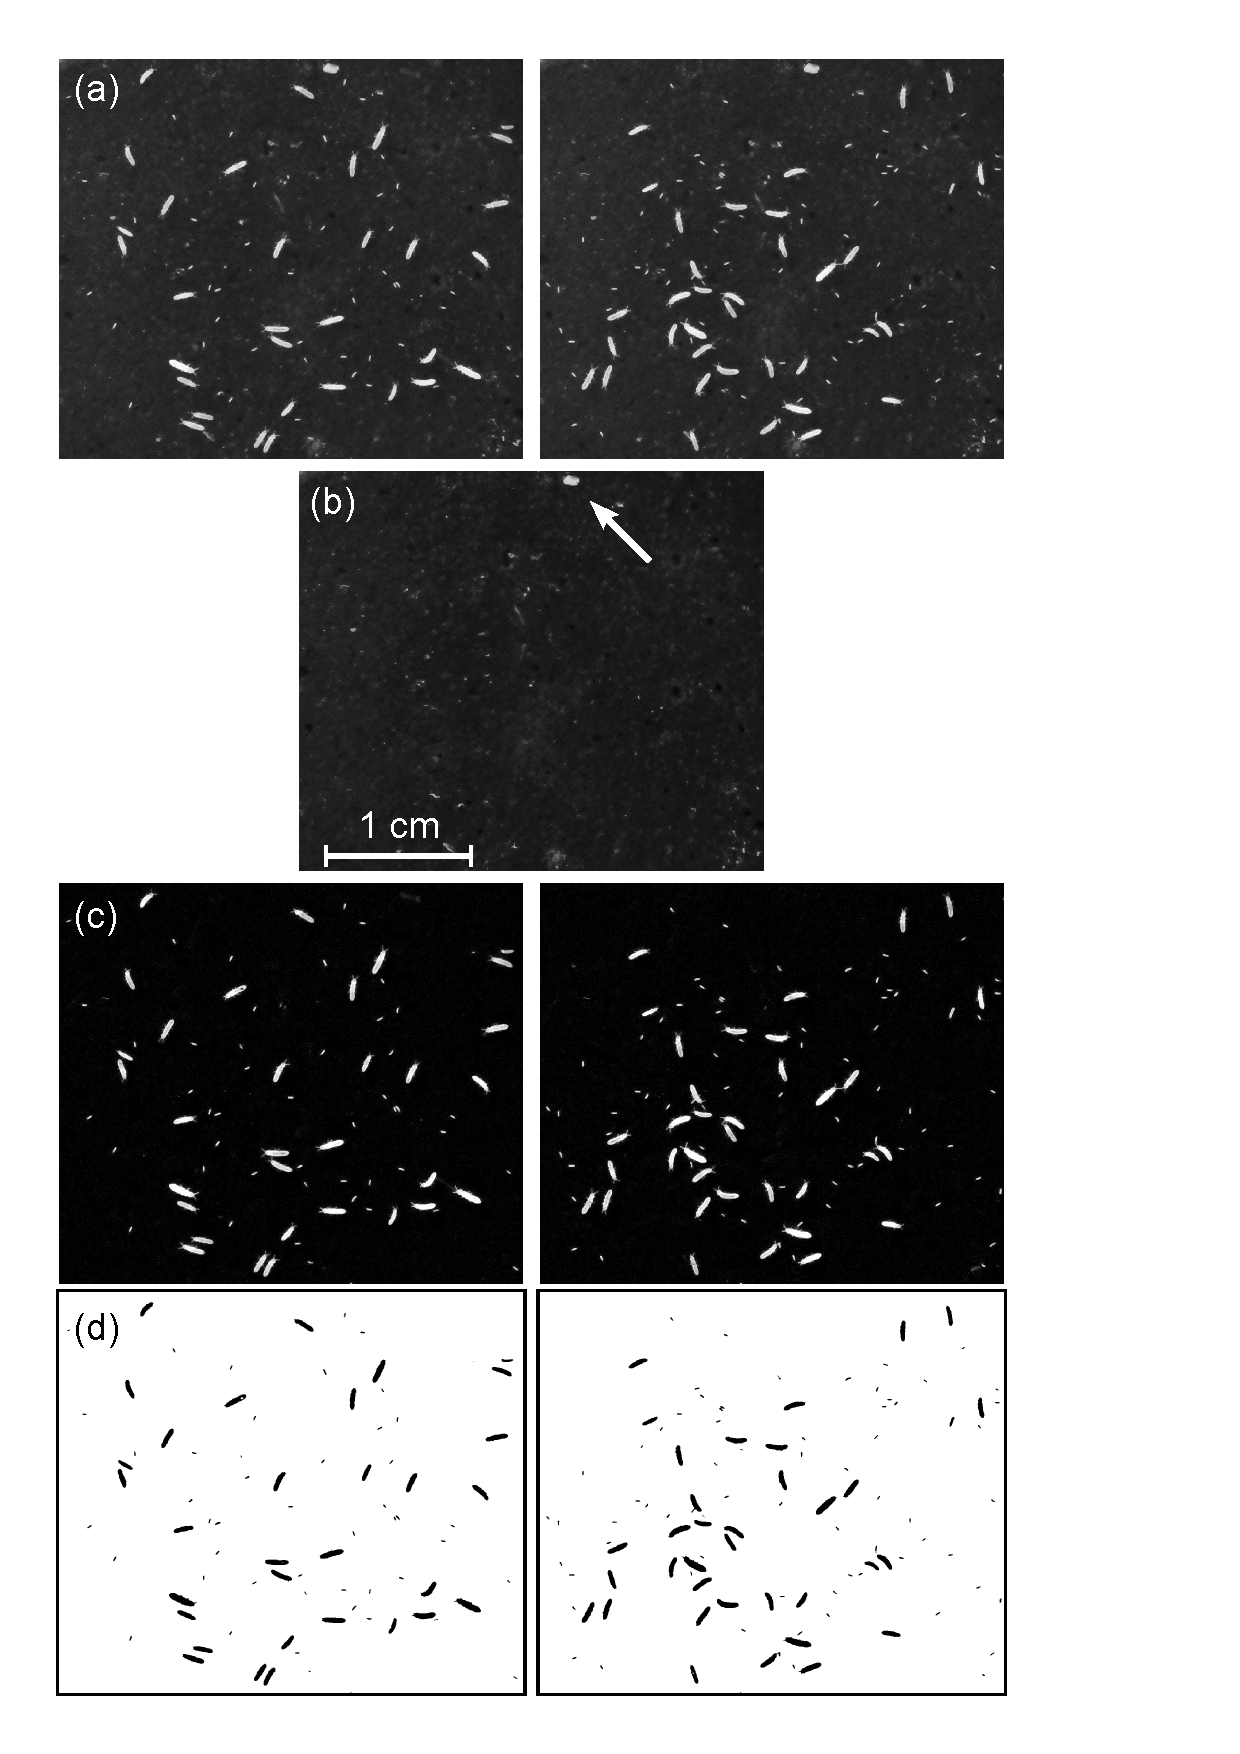
\includegraphics[width=0.55\textwidth]{1_CorpsDeThese/Methodo/1_collemboles_etapes}
\caption[\lofimage{1_CorpsDeThese/Methodo/1_collemboles_etapes} Les étapes
de l'analyse d'image]{Les étapes successives de l'analyse d'image (exemple
d'une population de collemboles).
(a) Deux photos extraites de la série d'images. (b) Le fond de l'image
reconstruit. Chaque pixel est sélectionné comme étant le plus sombre de la
pile d'image. (c) On soustrait le fond (b) à l'image de départ (a) pour
retirer le fond immobile et révéler les éléments mobiles. Le point blanc
(flèche) a été éliminé. (d) Après sélection de la limite d'intensité, on
peut compter et mesurer facilement chacune des particules.}
\label{fig:photoetapes}
\end{center}
\end{figure}



Le principe de base de la méthode développée consiste à comparer des plusieurs
photographies du même microcosmes prises à quelques secondes d'intervalle, en
gardant l'ensemble du dispositif immobile. Cela permet d'obtenir une série
d'image de la même population où seuls les éléments mobiles au cours de la prise
de vue différent entre les images. Généralement, trois à cinq photos sont
suffisantes pour que tous les individus vivants aient été mobiles entre au
moins la première et la dernière photo de la série (Figure
\ref{fig:photoetapes}a).

Au cours de nos expériences, l'ensemble des photos ont été prises avec un
appareil photo réflex piloté par ordinateur (Nikon D300 et
CameraControlPro\textcopyright). Il est également important de disposer d'un
éclairage stable afin que les conditions d'éclairage des prises de vue soient
constantes entre toutes les photos. Nous avons utilisé des ampoules à LED afin
de limiter le risque de fluctuation d'éclairage au cours du temps. 

Une fois la pile d'image obtenue, pour chacune des positions, on sélectionne
dans la pile d'image le pixel le plus sombre à cette position. Les collemboles
étant clairs sur un fond sombre, on reconstruit ainsi une image composite qui
contient uniquement les éléments immobiles au cours de la prise de vue (Figure
\ref{fig:photoetapes}b).
Ainsi, il suffit que tous les pixels de l'image soit au moins une fois sans collembole
dans la série de photos pour que l'image composite représente fidèlement le fond
de la boite. Si un élément clair (une mue par exemple) est présent sur le
substrat, s'il est strictement immobile, il sera également sélectionné comme
fond de l'image (flèche sur la Figure \ref{fig:photoetapes}b). 
On peut alors soustraire le fond immobile de chacune des photos de départ pour
obtenir des images ne contenant que les éléments immobiles (Figure
\ref{fig:photoetapes}c). 

La dernière étape consiste alors à convertir les images en image 8-bits (256
niveaux de gris), et de sélectionner le niveau de gris qui permettra de faire la
différence entre les collemboles et le reste de l'image (limite d'intensité,
Figure \ref{fig:photoetapes}d). Cela crée une image 2-bits (noir ou blanc) sur
la quelle le logiciel ImageJ peut détecter les contours et mesurer les
particules (pour nous les collemboles).

La série d'opération décrite a ensuite été automatisée dans un plugin pour
ImageJ où la plupart des étapes sont automatiques afin de bénéficier d'un
rendement accru dans le traitement des images.

\subsection{Fiabilité de la méthode}

Nous avons testé notre méthode sur différents critères \begin{enumerate*}[label=(\roman*), before=\unskip{ : }, itemjoin={{ ; }},
itemjoin*={{ ; et }}] 
\item le nombre d'image nécessaires au calcul du fond
\item la répétabilité de la mesure de la structure de la population
\item la fiabilité du dénombrement de la population
\end{enumerate*}

\begin{figure}[!ht]
\begin{center}
\includegraphics[width=0.80\textwidth]{1_CorpsDeThese/Methodo/6_Plugin_multiP}
\caption[\lofimage{1_CorpsDeThese/Methodo/6_Plugin_multiP} Analyse de la
fiabilité]{Analyse de la fiabilité de la méthode de mesure. (a) Biosurface
totale de collemboles mesurée ($mm^2$) en fonction du nombre de photos utilisés
pour constituer le fond. (b) Distribution en taille d'une même population de
collemboles mesurée quatre fois indépendemment par deux utilisateurs
différents, la ligne rouge représente un modèle général additif qui ne montre
aucune différence significative entre les photos ou les séries de mesure. (c)
Biosurface en fonction du nombre d'individus (cercles) comptés automatiquement,
les flèches montrent le nombre d'individus comptés à la main, la ligne
pointillée représente une régression linéaire sur les premiers points de mesure.
(d) Comparaison du nombre d'individus comptés automatiquement et à la main. }
\label{fig:photofiabi}
\end{center}
\end{figure}

\subsubsection{Nombre d'image pour le calcul du fond}

Dix populations contenant des densités croissantes d'individus de $0.25$ à
$0.5mm$ ont été prises en photos dans les conditions décrites précédemment avec
des séries de 20 photos. La biosurface d'individus (surface occupée sur la photo
par les individus) a été compté pour chacune des dix populations en utilisant un
nombre croissant d'image pour le calcul du fond. Si la densité d'individus est
élevée dans la populations, un plus grand nombre de photos sont nécessaires pour
obtenir une image fidèle du fond de la boite, dépourvu d'individus mobiles qui
auraient du être éliminés. Bien qu'à faible densité le nombre de photo utilisées
pour le fond de la boite ait peu d'effet sur la mesure de densité, à forte
densité, les mesures répétées dans les populations montrent que la biosurface
mesurée augmente avec le nombre d'image utilisées pour le fabriquer le fond
(Figure ref{fig:photofiabi}a). Il faut un minimum de quatre à cinq images à très
fortes densités pour obtenir une mesure fiable. En revanche il n'est pas
nécessaire d'utiliser plus que six images pour établir le fond, la mesure
de densité n'est pas améliorée. 

\subsubsection{Répétabilité de la mesure de la structure en taille}

Quatres jeux de cinq photos ont été analysés. Deux utilisateurs différents ont
prix chacun deux jeux de photos à quelques minutes d'intervalle pour assurer
l'indépendance des mesures. Les distributions en taille mesurées pour chacun des
quatre jeux de photos sont alors superposés et comparés en utilisant un modèle
additif autorégressif (Figure \ref{fig:photofiabi}b). Les quatre distributions
obtenues se recouvre largement et aucune différence significative n'a pu être
mise en évidence. Notre méthode permet donc une mesure fiable et répétable de la
structure en taille de la population.

\subsubsection{Fiabilité du dénombrement}

Le nombre de particule et leur surface ont été comptés avec la procédure
automatique sur dix populations de densité croissante. Ces mesures automatiques
sur des jeux de vingt photos ont ensuite été comparées à des comptages manuels
du nombre d'individus. 

En dessous de 1000 individus, notre méthode de comptage d'individus présente une
remarquable fiabilité (Figure \ref{fig:photofiabi}d). Au delà de cette densité,
le nombre d'individus comptabilisés par la méthode automatique est de plus en
plus sous-estimé par rapport au comptage manuel. En effet, lorsque la densité
augmente, de plus en plus d'individus se touchent sur les photos et sont alors
détectés comme une seule grosse particule. La biosurface devient alors un
meilleur proxy pour le nombre d'individu à supposer que tous les individus aient
une taille similaire, ce qui est le cas dans cet exemple. On peut alors projeter
la relation entre biosurface et nombre d'individus obtenue à faible densité pour
les forte densité et ainsi connaitre le nombre d'individus en mesurant la
biosurface (Figure \ref{fig:photofiabi}c).

\subsection{En conclusion}

En conclusion, cette méthode présente une grande fiabilité et permet d'accéder à
moindre coût à plusieurs mesures au sein des populations de collemboles pour une
perturbation minimale. Pour cette thèse, cette méthode permet d'accéder au
nombre d'individus ainsi qu'à la longueur corporelle et la biosurface de chacun
des individus, donnant ainsi une mesure de la structure des populations. 

De plus l'implémentation automatisée de la méthode permet de mesurer un grand
nombre de population dans un temps réduit. Une centaine de populations sont
ainsi dénombrées en environ trois heures sur un ordinateur dual-core cadencé à
$2.5GHz$ (à raison de $20$ à $30s$ par jeux de 5 photos).

D'autre part, cette méthode peut également être appliqué à d'autres organismes
ou systèmes expérimentaux. Plusieurs exemples d'utilisation sont décrits en
détail en annexe (voir Chapitre \ref{chap:bpsensor}).

\section{Méthode de représentation graphique}

Notre méthode automatisé d'analyse d'image pour le dénombrement et la mesure de
la structure en taille des populations de collemboles nous permet d'accumuler
rapidement un grand nombre de données. Précisément, à chaque date de mesure nous
disposons pour chacune des populations étudiées le nombre d'individus, et pour
chacun des individus sa taille corporelle ainsi que sa biosurface. Au cours de
nos expérimentations, nous avons été amenés à suivre plusieurs dizaines de
populations durant plusieurs dizaines de semaines.


\selectlanguage{french}
\part{Résumé des travaux de thèse}


%% Chaque section est un résumé en français d'un papier présent dans les annexes.

\chapter[SP]{Accès à la ressource taille dépendant et compétition par interferece : Analyse de séries temporelles longues de populations de collemboles \textit{Folsomia candida}}



\chapter[Interférence vs. exploitation et dynamique des populations
structurées][Interférence et populations structurées]{Interférence vs.
exploitation et dynamique des populations structurées}

\vspace{2cm}
\begin{Spacing}{1}
\texttt{
Le Bourlot, Vincent, Thomas Tully and David Claessen, "Interference versus
Exploitative Competition in the regulation of Size-Structured Populations"\\
under review at The American Naturalist
}
\end{Spacing}

\section*{Résumé}
%\addcontentsline{toc}{section}{Résumé}


\lettrine[lines=3]{L}{a compétition}  est un des facteurs principaux dans la
régulation de la dynamique des populations et des communautés. Son effet peut
être soit direct entre plusieurs individus via la compétition par
interférence, ou médiée par la ressource dans la compétition par
exploitation. L'impact de la compétition par exploitation sur la dynamique des
populations a déjà été largement étudié, tant d'un point de vue empirique
que théorique, mais les effets de la compétition par interférence restent
quant à eux mal compris. Nous étudions ici les effets de différents niveaux
de compétition intra-spécifique par interférence sur la dynamique d'une
population structurée en taille. Nous basons notre étude sur un modèle
ressource -- consommateur physiologiquement structuré prenant en compte des
interactions directes entre les individus, autorisant ainsi un gradient de
compétition depuis une compétition purement par exploitation à une
compétition totalement dominée par l'interférence. Nous paramétrons notre
modèle en utilisant des données issues de suivis expérimentaux de populations
de collemboles \textit{Folsomia candida}. Notre modèle prédit une variété de
dynamiques possibles suivant le niveau de compétition par interférence
imposé. A un faible niveau d'interférence, notre modèle se comporte de
manière similaire au modèle classique de Kooijman et Metz. Un niveau plus fort
d'interférence agit comme une force stabilisatrice sur les cycles de
générations causés par les juvéniles. A niveau intermédiaire, des géants
émergent dans la populations et commencent à la dominer. Enfin, à un niveau
très élevé d'interférence, un nouveau type de cycle apparaît que l'on
appelle cycles causés par l'interférence. Nos résultats théorique permettent
d'apporter un nouvel éclairage dans l'interprétation des dynamiques de la
structure en taille des populations de collemboles élevées au laboratoire.

\section{Introduction et méthodologie}



\chapter[SM]{Résilience de la structure en taille de popualtions de collembole \textit{Folsomia candida} modification expérimentale de la structure en taille et impact sur la dynamique de la population}


\chapter[FIP]{De l'individu à la population: quand la densité dépendense casse la règle taille~--~température}
\label{chap:fip}









\partimage[width=\textwidth]{FigParts/writing3}
\part{Conclusion Générale}

\chapter{Conclusion générale}

\section{Principaux résultats de la thèse}

Au cours de cette thèse, nous avons exploré certains détails de la dynamique des
populations structurées, aussi bien d'un point de vue expérimental que
théorique.
Nous avons porté une attention toute particulière aux rôles que jouent les
interactions taille-dépendantes entre individus dans l'établissement de ces
dynamiques, d'abord en observant des populations expérimentales de Collembole
\textit{Folsomia candida} sur le long terme pour en analyser les dynamiques en
fonction de leur structure en taille, puis en modélisant les interactions
tailles dépendantes entre individus dans un modèle physiologiquement structuré,
et enfin en manipulant la structure de plusieurs populations et en observant les
comportements d'accès aux ressources. Nous nous sommes ensuite intéressés à
l'effet de l'environnement, via la température ambiante, sur les interactions
taille-dépendantes et les répercussions sur la dynamique des populations.

Dans ce dernier chapitre, nous reviendrons sur les principaux enseignements
méthodologiques ainsi que théoriques et expérimentaux que l'on peut tirer de ces
travaux.

\subsection{Développements méthodologiques}

J'ai choisi de revenir ici sur quelques développements méthodologiques réalisés
au cours de cette thèse car ils n'ont pas seulement occupé une grande partie de
mon travail, mais ont également été une source d'inspiration et se sont
également révélés indispensables au bon déroulement de ces travaux.

\subsubsection{Le phénotypage haut débit}

Le développement de la méthode d'analyse d'image pour le dénombrement et la
mesure de la structure des populations a été un élément clé qui a rendu possible
ce travail. Cette méthode de suivi des populations a été initialisées par Thomas
\textcites{tully2004a} au cours de sa thèse, puis reprise en développée par
François \textcites{mallard2013b} et moi-même pendant plusieurs années avant de
faire l'objet d'un chapitre dans un ouvrage du CNRS \autocites{le-galliard2012a}
et d'une publication \autocites{mallard2013a}.

La méthode développée a notamment rendu possible la réplication des expériences
dans une mesure que l'on n'aurait pas pu atteindre en dénombrant manuellement
les populations. C'est une méthode fiable qui permet à peu de frais d'accéder à la
structure en taille d'une population (et donc à la densité dans les différentes
classes de taille) en peu de temps et de façon très peu voir pas du tout
intrusive.

Cette méthode a été développée et appliquée à des populations de collemboles,
mais est susceptible d'être facilement transposée à d'autres systèmes
expérimentaux comme nous l'avons décrit \autocites{mallard2013a}, ce qui lui
donne un grand intérêt pour l'écologie expérimentale et l'étude des traits
d'histoire de vie.

\subsubsection{Diagrammes structure-temps}

Le travail présenté dans cette thèse n'aurait pas non plus été possible sans
l'utilisation de la représentation graphique en diagrammes structure-temps et
des outils d'analyse graphique associés. En effet, cette technique simple de
représentation des données a permis de rendre cohérentes des données d'une
grande richesse dans les quelles il aurait été facile de se perdre.

Bien que cette méthode de représentation ne soit pas nouvelle elle n'a été à ce
jour que très rarement utilisée pour représenter des dynamiques de populations
structurées. Nous pensons que son application à des séries temporelles
structurées permettra de mettre en évidence des phénomènes qu'il était jusqu'à
présent difficile de décrire. Cette représentation remplit les critères
d'excellence des représentations graphiques en statistique décrits par
\textcites{tufte1990a} en condensant une grande quantité d'information sur un
petit espace de représentation, sans déformer les données et en révélant
plusieurs niveaux de détails en une seule fois, des structures fines à la vue
d'ensemble \autocites{tufte2001a}. Avec le développement des méthodes
automatisées telles que celle présentée dans cette thèse \autocites[voir aussi
][]{le-galliard2012a} et la croissance toujours accélérée des bases de données
(``big data''), ce type de méthode devrait à l'avenir se démocratiser, autant en
écologie des populations que dans des domaines plus variés comme en démographie
humaine, en épidémiologie, dans les enquêtes d'opinion, d'usage, \textit{etc}.
(Voir Annexe \ref{Chap:STDiag}).

\subsection{Taille corporelle et populations structurées}

Au-delà des apports méthodologiques, les travaux présentés dans cette thèse
répondent à des questions fondamentales en écologie des populations quant aux
rôles des interactions entre individus au sein d'une population dans la
régulation de sa structure et de sa dynamique, et à la place qu'occupe la taille
corporelle des individus dans la détermination de ces interactions.

\subsubsection{Taille corporelle et compétition par interférence}

Un premier résultat qui ressort de cette étude est l'importance de la différence
de taille corporelle entre individus dans la régulation de la dynamique de nos
populations expérimentales. Nous avons pu montrer au cours des différentes
expériences menées et suivis de populations que la présence de classes de
tailles différentes en densités différentes avait un impact direct sur la
dynamique que l'on pouvait observer, tant à court terme qu'à long terme.
La présence d'individus de grande taille notamment s'est montré un critère
déterminant dans les dynamiques observées dans les différentes populations.

En observant plusieurs populations dans les mêmes conditions, nous avons pu
montrer que les différentes structures en taille observées sont en nombre
limité, et peuvent être regroupées en quatre grandes catégories. Ces catégories
de structures, que l'on a appelé structures types, se différencient par
l'abondance des juvéniles, et la taille et l'abondance des adultes.
Un de ces types de structures est particulièrement remarquable par le fait qu'il
contient trois modes séparés dans la distribution de la taille (structures
de types 4), contrairement aux trois autres qui n'en contiennent que deux. Cette
structure type n'a par ailleurs été observée qu'à une seule température
(21$\degres$C) chez un seul des deux clones étudiés (HA), et cela quel que soit
l'expérience menée. Dans les populations montrant cette structure, la dynamique est conditionnée par les adultes les plus
grands. Leur présence contraint le reste de la population, empêchant notamment
la plupart des recrutements. Leur disparition, progressive ou brutale, permet la
croissance des juvéniles et d'une partie des adultes de plus petite taille.

Malgré ces particularités des structures de type 4, le point commun avec les
autres types de structure est la présence d'adultes à une taille corporelle
stable nettement supérieure à la taille à maturité, ce qui est contraire aux
prédictions des modèles de populations structurées régulées par compétition
intra-spécifique par exploitation
\autocites{kooijman1984a,de-roos1997a,de-roos2003a,de-roos2003b}.

L'observation des dynamiques de court terme dans ces populations (Chapitre
\ref{chap:sp} Section \ref{sec:shortterm}) a permis de démontrer que ces adultes
de taille relativement élevée jouaient un rôle déterminant dans les dynamiques
de la structure des populations. Leur disparition progressive ou brutale
coïncide de façon quasi systématique avec un événement de recrutement de
juvéniles dans les classes adultes. La perturbation de la structure des
populations dans une seconde expérience a permis de renforcer le lien de
causalité entre la présence des adultes et la croissance ou non des juvéniles.
En effet, retirer l'ensemble des adultes d'une de nos populations de collemboles
provoque un événement massif de recrutement alors que ne retirer qu'une partie
des adultes ne permet qu'à peu de juvéniles de recruter.
Lorsque plusieurs classes de taille coexistent chez les adultes, le retrait des
plus grands, même moins nombreux, provoque un événement de recrutement plus
important que le retrait des plus petits. Retirer des individus de grande taille
permet donc de rendre la possibilité aux juvéniles de grandir et d'atteindre la
maturité.

Cette domination des adultes sur la dynamique de la structure de nos populations
s'explique par la domination qu'ils exercent sur l'accès à la ressource fournie.
Cette hypothèse, issue de l'observation des séries temporelle de la structure
des populations, a été confirmée par l'observation des comportements d'accès à
la ressource et la mesure du biais de taille dans cet accès. Par ces mesures, on
a pu montrer une sur-représentation systématique des individus les plus grands
au contact ou aux abords de la pastille de ressource. Cette pastille de
ressource étant très localisée par rapport à l'environnement de vie des
Collemboles, il est alors possible pour la minorité d'individus les plus grands
de monopoliser la ressource et d'en restreindre l'accès aux plus petits. Ces
derniers ne pouvant se nourrir ne peuvent alors pas se développer et restent
dans un stade juvénile jusqu'à ce que le nombre d'adultes diminue suffisamment
pour que la ressource devienne à nouveau accessible.

Ce comportement des individus les plus grands repoussant les plus petits aux
abords de la ressource et ses conséquences sur la dynamique de la structure
montre l'existence d'une compétition par interférence, parfois de forte
intensité, dans nos populations de collemboles. Cette compétition par
interférence contre balance l'avantage énergétique que possèdent les petits
individus et permets ainsi aux plus grands de survivre et de dominer la
population.

\subsubsection{Compétition par interférence et dynamique des populations
structurées}

Nous avons montré le rôle de la compétition par interférence dans la régulation
de nos populations expérimentales structurées en taille, et notamment comment
elle permettait la survie d'individus de grande taille, et parfois de géants
très longévifs qui, même en petit nombre, dominent le reste de la population
(voir par exemple Figure \ref{fig:SP1}).

Afin d'étudier plus avant les conséquences de l'existence d'une compétition
intra-spécifique par interférence sur la dynamique d'une population structurée,
nous avons repris le modèle classique de dynamiques de populations
physiologiquement structurées développé pour les Daphnies
\autocites{kooijman1984a}. Nous avons adapté ce modèle à notre système en le
paramétrant pour les collemboles, ce qui a été possible car le cycle de vie des
collemboles présente des similarités avec celui des daphnies dans le sens où ils
ont une croissance continue, et les juvéniles et les adultes ont la même
apparence et partagent la même niche, ne se différenciant que par la taille.
Nous avons ensuite étendu le modèle pour y intégrer une représentation des
interactions directes entre individus dépendante des tailles respectives des
adversaires. Nous avons alors été en mesure de modéliser différents niveaux de
compétition par interférence pour en observer les conséquences sur la dynamique,
comparées à un modèle avec de la compétition par exploitation seule. Ce modèle
présente l'avantage de rester simple tout en regroupant les aspects principaux
de la compétition par interférence.

Nous avons montré avec ce modèle que la présence de la compétition par
interférence intra-spécifique pouvait avoir différentes conséquences en fonction
de son intensité. En l'absence d'interférence, la théorie existante sur les
modèles PSP décrit déjà les dynamiques prédites, et notamment la présence de
cycles de génération à faible mortalité, et l'effet stabilisant d'une forte
mortalité. Un premier résultat de ce modèle est l'effet stabilisant de la
compétition par interférence lorsqu'elle est à niveau intermédiaire. Si son
intensité est suffisante, la compétition par interférence vient contrebalancer
l'avantage qu'ont les juvéniles par la compétition par exploitation, et produit
ainsi un effet similaire à l'augmentation de la mortalité basale en amortissant
les cycles de génération. On obtient alors une structure de population stable
similaire à celle que l'on aurait sans interférence avec une forte mortalité
basale.

L'augmentation de la compétition par interférence a aussi pour effet de faire
augmenter la capacité des individus les plus grands de la population à accéder à
la ressource. Lorsque cette capacité est suffisante, les individus, qui jusque
là arrêtaient de grandir à une taille proche de la taille à maturité, peuvent
alors reprendre leur croissance, et atteignent des tailles importantes, proches
de leur maximum physiologique possible. Il est intéressant de noter que cela se
produit aussi bien dans une dynamique stable que cyclique. Une fois le seuil
d'interférence permettant la survie des géants dépassé, ceux-ci seront toujours
présents dans les populations et les domineront tant que l'interférence reste
élevée.

Enfin, à un niveau très élevé, la compétition par interférence donne un tel
avantage aux adultes de grande taille que la dynamique est déstabilisée dans un
nouveau type de cycles. Ces cycles sont également des cycles de génération, mais
de beaucoup plus grande amplitude et plus longue période. De plus contrairement
aux cycles observés en l'absence d'interférence, ce sont cette fois les adultes
qui dominent la dynamique et génèrent les cycles.

La présence des individus de grande taille et les nouveaux cycles décrits
présentent des similarités avec d'autres phénomènes déjà étudiés dans les
populations structurées, notamment le cannibalisme, ou la compétition
différentielle entre adultes et juvéniles, mais apporte une nouvelle explication
aux dynamiques observées, parfois plus parcimonieuse que celles précédemment
proposées. Ce modèle de dynamique de populations structurées, régulées par la
compétition par interférence, permet donc de compléter les résultats
préexistants sur la compétition par exploitation et le cannibalisme comme
mécanisme régulateur des populations structurées.

Dans nos populations expérimentales, nous pensons que la compétition par
interférence suffit à expliquer les structures bimodales observées. La Figure \ref{fig:Concl0} résume
le rôle que jouerait la compétition par interférence. En interférant avec les plus petits
individus, les adultes de grande taille les empêchent d'accéder à la ressource.
Le taux de croissance des petits individus devient alors rapidement négatif avec
la taille, et ils arrêtent de grandir. Pendant ce temps, les adultes sont très
compétitifs et ont une longue survie grâce à leur accès facilité aux ressources.
Cependant, du fait de la stochasticité des populations expérimentales, certains
juvéniles peuvent ponctuellement avoir accès à la ressource, et leurs taux de
croissance deviennent alors positifs pendant une brève période. Ils parviennent
ainsi à s'échapper et rejoindre la cohorte des adultes. 

\begin{figure}[!ht]
\begin{center}
\includegraphics[width=1\textwidth]{Conclu/Interf0}
\caption[\lofimage{Conclu/Interf0}Rôle de l'interférence dans la
structuration bimodale]{Rôle de l'interférence dans la
structuration bimodale de nos populations expérimentales de Collemboles.}
\label{fig:Concl0}
\end{center}
\end{figure}


\subsection{Les effets de la température}

Au cours d'une dernière expérience, nous avons comparé des normes de réactions à
la température, mesurées sur des individus isolés et dans des populations. Nous
avons pu montrer que les processus de régulation des populations tels que la
compétition par exploitation et par interférence, sont soumis aux effets de
l'environnement et notamment à la température ambiante à laquelle se trouve la
population.

Nous avons montré en introduction que la température est un facteur abiotique
connu pour ses effets sur les individus, les populations et les communautés.
Chez les organismes ectothermes, en agissant sur le métabolisme, un changement
de température affecte toute la physiologie de l'individu, ce qui se répercute
sur la gestion de l'énergie, le comportement, la croissance et l'investissement
reproducteur de ce dernier. Ces répercussions en cascades ont ensuite un impact
fort sur la dynamique des populations concernées, qui en retour est elle-même
susceptible d'affecter la communauté.

Plus précisément, nous avons montré dans le cas des collemboles que
l'augmentation de la température a un effet prévisible sur les individus isolés,
provoquant notamment une réduction de la taille asymptotique lors d'une
augmentation de température, conformément à la règle taille-température
\autocites{angilletta2009a}. En revanche, dans les populations, l'effet d'une
température plus élevée se retrouve confronté aux mécanismes de compétition
intra-spécifique, le résultat sur la dynamique des populations et leurs
structures est alors moins facile à prévoir. Nous avons montré que dans une
gamme intermédiaire de réchauffement, la température provoque une diminution des taux
de croissance et des tailles corporelles adultes, mais dans une bien moindre
mesure que chez les individus isolés, les effets de la température sont en
partie tamponnés par les mécanismes de densité dépendance (Figure
\ref{fig:Concl1}).

\begin{figure}[!ht]
\begin{center}
\includegraphics[width=1\textwidth]{Conclu/TempSizeRule}
\caption[\lofimage{Conclu/TempSizeRule}Règle Taille-Température en
population]{Effet de la densité dépendance sur la règle taille température en
population}
\label{fig:Concl1}
\end{center}
\end{figure}

De façon plus étonnante, dans des conditions de température élevée
($26\degres$C), nous avons montré que les tailles adultes ne suivent plus la
règle taille-température, même après avoir corrigé les mesures pour les effets
de la densité d'individus. Il semblerait alors qu'il soit plus intéressant pour
les individus d'investir dans la croissance et d'atteindre des tailles
supérieures, malgré les désavantages liés à la température. Nous proposons pour
expliquer cela l'inversion des mécanismes de régulation dans les populations
entre compétition par exploitation et compétition par interférence (Figure
\ref{fig:Concl2}). Plus précisément, à température basse ou intermédiaire, la
compétition par exploitation aurait une plus grande importance que la
compétition par interférence dans la régulation des populations. Nous pensons
également que l'intensité des compétitions par exploitation et par interférence
augmente avec la température, mais que la compétition par interférence augmente
plus vite que la compétition par exploitation, notamment à cause de
l'augmentation de l'activité et du besoin en nourriture par unité de temps.
Ainsi, à partir d'une température critique, le désavantage d'une grande taille
lié à la température serait sur-compensé par l'avantage lié à la supériorité par
interférence. Malgré la température élevée, les individus de grande taille
gagnant un accès quasi-exclusif à la ressource deviennent alors dominant dans
les populations.

\begin{figure}[!ht]
\begin{center}
\includegraphics[width=1\textwidth]{Conclu/TempSizeRule2}
\caption[\lofimage{Conclu/TempSizeRule}Température et importance des
compétitions par exploitation et interférence]{Température et importance des
compétitions par exploitation et interférence}
\label{fig:Concl2}
\end{center}
\end{figure}


En plus de son effet direct sur les individus, la température a donc également
un effet sur les interactions entre les individus et modifie les rapports de force
compétitifs entre individus de petite et de grande taille. En modifiant ces
rapports de force, la température affecte la dynamique des populations non
seulement via ses effets sur les individus, mais également via ses effets sur
les mécanismes de compétition.

\subsection{Compétition par interférence dans les populations naturelles}

Les différents résultats de ces travaux montrent l'importance de considérer la
compétition par interférence dans la description, la compréhension et la
prédiction de la dynamique des populations structurées en taille. La taille
individuelle est un élément structurant extrêmement répandu dans les populations
naturelles. Il est donc important de pouvoir reconnaître dans ces populations
les effets de la compétition par interférence. Les données expérimentales
présentées dans ces travaux rendent assez facile la détection de la compétition
par interférence et l'analyse de son rôle dans la dynamique des populations.
Malheureusement, ces données très complètes sont difficiles voire impossible à
recueillir dans la nature. Il faut donc pouvoir se baser sur des critères plus
simples permettant de proposer la compétition par interférence comme mécanisme
participant à la régulation des populations.

A cette fin, notre étude théorique nous a permis de proposer des critères de
recherche pour identifier le rôle de la compétition par interférence. Le premier
des critères est l'émergence d'individus géants dans les populations.
Ces individus ont une durée de vie très longue comparée aux individus plus
petits, et peuvent dominer les dynamiques des populations. Bien que plusieurs
mécanismes puissent engendrer des géants (cannibalisme, niche écologique
spécifique, \ldots), leur présence est un premier indice qui, associé aux
critères suivants, pointe vers la compétition par interférence.

Si les données recueillies le permettent, l'observation de courbes de croissance
en deux temps avec une stagnation (proche de la maturation) suivie d'une reprise
de croissance avant de converger vers une taille asymptotique élevée est
également un indice d'une compétition par interférence relativement intense. Ce
ralentissement de croissance (goulet d'étranglement de la croissance) provoque
alors des distributions de taille très asymétriques, fortement biaisées en
faveur des juvéniles dans le cas où la population est stable. Si la structure de
la population est cyclique avec de longues périodes au cours desquelles la
distribution est multi-modale, cela indique aussi un niveau élevé de compétition par
interférence.

Enfin, dans le cas où les données ne permettent pas l'observation détaillée des
courbes de croissance ou de la dynamique temporelle de la structure des
populations, la mesure du temps de génération comparée à la durée des
oscillations dans des populations périodiques (les oscillations sont mesurées en
comptant l'abondance totale de la population) permet également de proposer la
compétition par interférence comme mécanisme régulateur si le ratio des deux
grandeurs est entre 1 et 2. Si ce ratio est inférieur à $1$, les oscillations
correspondent à des ``single generation cycles'', et probablement des cycles
dirigés par les juvéniles qui seraient donc régulés par de la compétition par
exploitation. A l'inverse, si le ratio est entre 2 et 4, il s'agit alors de
cycles dit ``delayed feedback cycles'', et enfin au delà de 6, de cycles
ressource-consommateur ou prédateur-proie \autocites{murdoch2002a}. Ce dernier
indice n'apporte pas la même fiabilité que les critères précédents, mais peut
permettre de poser l'hypothèse de la compétition par interférence et de diriger
les efforts de récolte des données nécessaires à l'identification de son rôle,
telles que les courbes de croissances individuelles ou les données détaillées de
structure au cours du temps.

\section{Hypothèses et limites}

Les résultats rapportés dans cette thèse sont issue de travaux expérimentaux et
théoriques. Comme tous les travaux de ce type, ils comptent leur lot de
limitations et d'hypothèses sous-jacentes. Nous allons tenter ici de les
expliciter afin de montrer comment en tenir compte et éventuellement les
contourner ou les lever dans de futurs développements.

\subsection{Approches expérimentales}

Les différentes expériences menées au cours de cette thèse ont consisté à
suivre des collemboles dans des conditions contrôlées. Les conditions d'élevages et de
mesure des populations entraînent quelques limitations qu'il est nécessaire de
mentionner.

\subsubsection{Conditions d'élevage}

Nos collemboles sont élevés dans des boites en plastique de cylindriques de
$5.1cm$ de diamètre, remplies d'un substrat en plâtre de $3cm$ permettant de
conserver l'environnement d'élevage à un taux de saturation en eau proche de $100\%$.
Les collemboles étant extrêmement sensibles à la dessiccation, ceci
constitue une première difficulté dans l'élevage et le suivi de populations de
collemboles. Cela nous oblige à surveiller régulièrement l'état de sécheresse
des boites d'élevage. En cas de boite sèche, la survie des collemboles n'excède
pas quelques jours, voir quelques heures à température élevée. Il est donc
essentiel de maintenir le taux d'humidité à son maximum pour éviter une
mortalité accrue des individus.

Une autre limite intrinsèque aux conditions d'élevage des collemboles est liée à
l'humidité nécessaire à la survie des collemboles. En effet, ces conditions
d'élevages et l'apport régulier de ressources est propice au développement de
moisissures sur la pastille de ressources et le fond de la boite. Durant leur
développement, ces champignons produisent de longs filaments dans lesquels les
collemboles se retrouvent piégés, et qui occupent parfois l'intégralité de la
pastille de ressource. Les collemboles sont alors incapables de se nourrir,
même s'ils sont toujours libres. Ces champignons provoquent donc une mortalité
accrue chez les collemboles, soit en occupant la ressource, soit en piégeant les
individus. L'invasion d'une boite par des champignons touche principalement les
individus les plus petits qui sont plus facilement piégés dans les filaments. La
mortalité accrue est donc plus grande chez les juvéniles. De plus, une fois
installés, il est extrêmement difficile de se débarrasser des moisissures. La
contamination d'une boite nécessite donc de transférer la population dans une
nouvelle boite d'élevage saine. Ceci peut alors entraîner des perturbations des
dynamiques, et est à l'origine de certains des événements catastrophiques
décrits dans le Chapitre \ref{chap:sp} (voir aussi Annexe \ref{Ann:SP}). Une
solution possible pour éviter la contamination par les moisissures peut être
d'utiliser des pastilles de nourritures traitées aux fongicides, mais
l'innocuité de ce traitement sur les collemboles n'est pas démontrée, et nous
avons choisi de ne pas l'utiliser dans nos expériences. A la place, nous avons
prêté une attention particulière à l'état de nos boites d'élevage qui ont été
nettoyées régulièrement. Malgré tout, il a été impossible de prévenir toute
contamination, et les populations atteintes ont été transférées dans de
nouvelles boites d'élevages dès que la contamination a été constatée.

Enfin, les conditions d'élevage utilisées constituent un milieu fermé sans
dispersion possible, et un milieu homogène. Ces conditions sont très différentes
des conditions naturelles de vie des collemboles ou le milieu est ouvert et à
trois dimensions (dans le sol). Les plus petits individus ont donc sans doute
accès à des interstices plus fins que les gros adultes. Et les interactions
entre individus sont probablement plus limitées grâce à une plus grande
possibilité des individus de s'éviter.

\subsubsection{Protocole expérimental}

Les suivis de populations mis en place au cours de cette thèse reposent sur un
apport hebdomadaire de nourriture sous la forme d'une pastille de levure mixée
dissoute dans de l'agar-agar. Sous cette forme, la pastille de nourriture occupe
très peu d'espace sur le fond de la boite d'élevage. Comme nous l'avons montré
dans cette thèse, la compétition pour l'accès à ces ressources est très forte et
le petit espace occupé par la pastille favorise les interactions et la
compétition par interférence. Ceci nous a permis de décrire les effets de ce
type de compétition sur les populations structurées, mais il est possible qu'une
partie des résultats décrits dans cette thèse soient la conséquence d'un niveau
extrême de compétition par interférence, dû au format de ressources choisi. Bien
que cela ne remette pas en cause les résultats décrits, il est nécessaire de
tenir compte de ces conditions particulières dans l'analyse des résultats
obtenus.

\subsubsection{Méthode de mesure}

Les populations suivies ont été dénombrées et leurs structures en taille
mesurées par la méthode semi-automatique décrite dans le Chapitre \ref{chap:method}
Section \ref{sec:bpsensor} (voir aussi Annexe \ref{Ann:bpsensor}).
Comme nous l'avons décrit, cette méthode est particulièrement fiable pour des
populations de moins de 1000 individus. Les populations suivies au cours des
différentes expériences ont atteint et parfois dépassé ces densités.
Il est alors possible que les mesures des tailles des populations soient
sous estimées. Plus précisément, lorsque la densité d'individus est très
élevée, les individus se touchent ou se superposent sur les photos utilisées
pour les dénombrements et les mesures de tailles. Ainsi, au lieu de compter
plusieurs individus de différentes tailles, l'algorithme d'analyse d'image
compte une seule particule de grande taille. Il est donc possible à très grande
densité que le nombre de juvéniles soit sous-estimé et le nombre de grands
adultes surestimé. Cependant, les comptages réguliers des boites et les mesures
moyennées sur plusieurs photos permettent d'augmenter la confiance dans les
mesures obtenues. De plus, malgré les incertitudes de mesure, la représentation
sous forme de diagramme structure-temps permet une représentation de la
dynamique de la structure qui rend apparent les dynamiques à courts termes et
les motifs sur le long terme en lissant en partie le bruit issue des données.

\subsection{Hypothèses du modèle}

L'analyse théorique du rôle de l'interférence dans la dynamique des populations
structurées repose elle aussi sur un certain nombre d'hypothèses dont il faut
tenir compte.

\subsubsection{Budget énergétique dynamique et allocation de l'énergie}

Une première hypothèse du modèle choisi repose sur la règle du budget
énergétique dynamique. Cette règle suppose notamment que l'absorption d'énergie
se fait proportionnellement à la longueur au carré de l'individu alors que son 
utilisation dans le métabolisme se fait proportionnellement à la longueur au
cube.
Les règles du budget énergétique dynamique ont été établies par \textcites{kooijman2000a}
d'après des travaux sur divers organismes. Chez les organismes étudiés,
l'ingestion de nourriture se fait par une bouche dont la taille est généralement
proportionnelle à la longueur de l'individu. Le taux d'ingestion de la
nourriture (et donc de l'énergie) dépend alors de la surface de la bouche, qui
est donc proportionnelle à la longueur au carré de l'individu. Le taux de
métabolisme dépend quant à lui du nombre de cellules présentes dans
l'organisme, ce qui dépend du volume de l'individu, essentiellement
proportionnel à sa longueur au cube. Bien que ces relations soient très
générales, elles n'ont pas été vérifiées précisément chez les collemboles à
cause des difficultés que posent la mesure de l'ingestion et de la consommation
de l'énergie chez ces organismes. Cependant, la grande généralité de cette
hypothèse fait que l'on peut l'appliquer également aux collemboles sans trop
de doute sur sa véracité.

Associé à ces hypothèses sur l'ingestion de l'énergie et sa consommation vient
l'hypothèse sur l'allocation du budget énergétique. Dans les travaux présentés
dans le Chapitre \ref{chap:amnat} (voir aussi Annexe \ref{An:AmNat}), nous
faisons l'hypothèse d'une allocation suivant la règle dite du $\kappa$. Cette
hypothèse se justifie notamment par le fait que les collemboles se reproduisent
tout au long de leur vie, même après avoir arrêté leur croissance. Cependant,
afin de vérifier que les résultats du modèles ne sont pas directement la
conséquence de cette règle d'allocation de l'énergie, nous avons testé une
seconde règle communément utilisée dans les modèles de populations structurées,
la règle dite de ``production nette'' (``net production model''). Sous cette
nouvelle hypothèse, l'énergie est d'abord allouée à la maintenance, et le reste
(s'il y en a) est divisé entre croissance et reproduction. Une conséquence
immédiate de cette règle est que l'arrêt de la croissance s'accompagne
nécessairement d'un arrêt de la reproduction. L'analyse du modèle dans le cadre
de cette règle est présentée dans les Supplementary Materials de
l'Annexe \ref{An:AmNat}, Section \ref{subsec:SupMat4}. Les résultats qualitatifs
en terme de types de dynamiques obtenues pour les différentes valeurs
d'interférence sont sensiblement identiques à ceux obtenus pour la règle du
$\kappa$. Ces résultats sont donc robustes et ne dépendent pas de la façon dont
l'énergie est répartie après acquisition.

\subsubsection{Reproduction continue}

Le modèle utilisé est une extension du modèle de \textcites{kooijman1984a}. Ce
modèle a été développé pour les Daphnies. Nous l'avons transposé aux Collemboles
après avoir vérifié les points essentiels assurant la validité du modèle (voir
Section \ref{subsec:SupMat1} des Supplementary Materials de l'Annexe
\ref{An:AmNat}).

Le modèle utilisé fait l'hypothèse d'une reproduction continue des individus.
Cependant, les collemboles se reproduisent par des pontes relativement
importantes tous les $10$ à $20$ jours suivant les conditions de température et
de densité des populations. A l'échelle des simulations réalisées (plusieurs
milliers de jours), cela peut être considéré comme quasiment continu,
cependant, il est possible que l'éclosion massive d'individus au même moment
entraîne des résultats différents comparés à une population où la reproduction
est strictement continue. Nous pensons toutefois que cette hypothèse de reproduction
continue, par opposition à la reproduction saisonnière de certains modèles de
poissons, notamment intégrant du cannibalisme
\autocites{claessen2000a,claessen2004a}, reste valide pour les collemboles
compte tenu des échelles de temps mis en jeu et du nombre d'individus présents
dans les populations. En effet, même si chaque individu se reproduit par des
pontes, la présence de nombreux adultes entraîne des éclosions quasi-continues
dans les populations.

\subsubsection{Représentation de la compétition par interférence}

Afin d'implémenter la compétition par interférence dans le modèle, et parce que
les données correspondantes n'étaient pas disponibles, nous avons dû faire une
première approximation et nous affranchir de la description explicite des
ressources et de leur consommation. Nous avons remplacé la dynamique de la
ressource par une dépendance directe de la population à sa propre densité (via
la fonction $\eta$). Cette approximation a été réalisée en supposant la
ressource à un état quasi stationnaire. Or, telle qu'elle est apportée dans les
populations expérimentales, la ressource n'est pas à un état quasi-stationnaire.
Il pourrait donc être intéressant de mesurer la consommation de la ressource
chez les collemboles afin de relaxer cette hypothèse et la réintégrer la
explicitement dans le modèle. L'apport ponctuel de ressource pourrait alors
 avoir un effet important sur les dynamiques produites par le modèle.

De plus, la compétition par interférence a été implémentée via la fonction de
compétition $C$ qui définit la supériorité d'un individu sur un autre en
fonction de leurs tailles relatives. Cette fonction a été choisie affine de
façon arbitraire avec une pente définie par l'intensité $I$ de la
compétition. Ce choix a été motivé par une volonté de simplicité de la
représentation. Mais ceci rend le modèle relativement théorique, et pas
forcément facilement applicable directement à d'autres organismes. De plus,
cette représentation ne prend pas en compte la possible dépense d'énergie par les
adversaires dans les interactions qui les opposent. Ainsi l'intérêt d'accéder à
la ressource pourrait être limité si la dépense d'énergie nécessaire au gain de
cet accès est supérieure à l'énergie gagnée. Ceci pourrait être pris en compte
en choisissant une forme plus complexe à la fonction de compétition qui
intégrerait par exemple une dépendance absolue à la taille en plus de la
dépendance à la différence de taille des adversaires. En supposant qu'un
individu plus grand dépense moins d'énergie qu'un petit au cours d'une
interaction compétitive, ou que des individus de tailles proches dépensent plus
d'énergie que des individus très éloignés, on pourrait également obtenir des dynamiques prédites différentes suivant les
niveaux d'interférence. Cependant, cela complexifie la modélisation, et
nécessiterait de nouvelles mesures pour choisir et calibrer les fonctions de
compétition. Or ces mesures sont potentiellement difficiles à réaliser
(notamment sur le collembole). De plus, malgré des différences quantitatives, les résultats
qualitatifs issus des simulations apportent des éléments d'explication aux
dynamiques observées dans les suivis de populations.
Nous pensons donc que le modèle décrit ici fournit une représentation simple et
minimaliste, mais pertinente des mécanismes de base de la compétition par
interférence et de ses conséquences sur la dynamique des populations
structurées.

\section{Perspectives futures}

Comme dans tout travail scientifique, les réponses aux questions soulevées dans
cette thèse ne s'arrêtent pas aux conclusions exposées dans ce chapitre.
Beaucoup de travail reste à faire pour comprendre pleinement les impacts de la
compétition par interférence sur la dynamique des populations. De même, des
zones d'ombre persistent quant à l'interaction entre la compétition par
interférence et les autres mécanismes de densité dépendance, ainsi qu'avec les
facteurs environnementaux comme la température, les facteurs climatiques plus
larges, la structuration de l'habitat, et tout autre facteur susceptible
d'influencer les individus et les populations. Afin de répondre au critiques
présentées précédemment et d'approfondir la connaissance du rôle de la
compétition par interférence dans la dynamique des populations, nous proposons
ici quelques pistes à la fois expérimentales et théoriques pouvant apporter de
nouveaux éclairages sur ces questions.

\subsection{Développement expérimental}

\subsubsection{Limiter les risques de contamination}

D'un point de vu expérimental, nous avons vu que plusieurs questions peuvent se
poser en lien avec le système développé au cours de cette étude. Un premier
impératif pour garantir la validité des résultats expérimentaux obtenus est de
trouver une méthode pour limiter au maximum les risques de contamination par les
moisissures. Une méthode permettant d'assainir les boites d'élevage consiste à
étaler un mélange d'argile et de charbon actif, inoffensif pour les collemboles,
sur le fond de la boite d'élevage. Cela fourni un meilleur environnement de vie
pour les individus tout en diminuant le risque de contamination. Cette méthode
ayant été développée après le lancement de nos suivis de populations, nous ne
l'avons pas utilisé dans nos expériences, mais elle a été testée et vérifiée par
François \textcites{mallard2013b} dans ses travaux de thèse et peut être
appliquée aux futures expériences.

\subsubsection{Répondre aux nouvelles questions}

Les travaux menés au cours de cette thèse ont soulevé de nouvelles questions,
en particulier concernant les liens entre le niveau de compétition par
interférence et les structures observées dans les dynamiques. Nous avons évoqué le fait que
le niveau élevé de compétition par interférence dans nos populations pouvait
être lié à la distribution très localisée de la ressource dans les boites
d'élevage. Un moyen de réduire le niveau de compétition par interférence et
ainsi de tester l'effet sur la dynamique de la structure des populations par
comparaison avec les résultats précédents, pourrait être de disperser la
nourriture apportée. Il s'agirait alors de fournir la même quantité de
nourriture mais occupant une surface plus grande sur le fond de la boite.
L'hypothèse est qu'en occupant une proportion plus grande de la surface de
la boite, l'accès aux pastilles de nourriture est plus facile pour l'ensemble
des individus, ce qui permettrait de diminuer les interactions pour y accéder,
tout en maintenant un niveau similaire de compétition par exploitation en
gardant la même quantité totale de nourriture. A l'inverse, un traitement où la
nourriture serait apportée en plus petite quantité mais plusieurs fois par
semaine afin de conserver la même quantité hebdomadaire permettrait de renforcer
la compétition par interférence. En effet, les pastilles seraient alors encore
plus petites que dans les conditions déjà testées, et les combats pour y accéder
plus intenses. Des expérimentations sont actuellement en cours pour vérifier ces
hypothèses.

De telles expériences à $21\degres$C permettraient de comparer les dynamiques
obtenues avec celles présentées dans le Chapitre \ref{chap:sp} (voir aussi
Annexe \ref{Ann:SP}). Ces comparaisons permettraient également de tester les
prédictions du modèle présenté dans le Chapitre \ref{chap:amnat}, et ainsi, en
faisant varier le niveau de compétition par interférence, vérifier si l'on peut
obtenir expérimentalement les différentes dynamiques produites par les
simulations (voir aussi Annexe \ref{An:AmNat}).
Cette validation expérimentale fournirait alors un argument en faveur de la
représentation simple de l'interférence proposée dans le modèle, et permettrait
également de tester les critères proposés pour reconnaître le rôle de
l'interférence.

Étendues aux différentes températures testées dans le Chapitre \ref{chap:fip},
ces expériences permettraient de vérifier l'hypothèse proposée d'une bascule
entre domination de la compétition par exploitation et par interférence entre
$21$ et $26\degres$C (voir aussi Annexe \ref{Ann:fip}). En effet, nous supposons
que les tailles plus grandes observées à $26\degres$C sont dues à une forte
intensité de l'interférence qui donne un avantage à des individus de grande
taille malgré le désavantage causé par une température élevée. En faisant varier
les niveaux d'interférence aux différentes températures, nous pourrions
vérifier s'il est possible d'observer un avantage aux petites tailles jusqu'à
$26\degres$C en diminuant l'interférence, ou au contraire, favoriser l'émergence
de géants avant $21\degres$C en l'augmentant. Ceci permettrait de valider notre
hypothèse et de confirmer les interactions entre processus démographiques et
effets de la température dans la régulation des populations.

Une autre piste envisageable pour étendre notre étude de la compétition
concerne l'impact de la température dans le cas d'un environnement changeant. On
pourrait modifier les températures d'élevage des collemboles avec différentes
fréquences et amplitude, et ainsi observer comment les variations de température
impactent la dynamique des populations par comparaison avec les résultats
obtenus dans le Chapitre \ref{chap:fip} pour des températures fixes (voir aussi
Annexe \ref{Ann:fip}). Ce type de protocole permettrait également d'étudier la
réponse des populations structurées à un environnement changeant, et plus
particulièrement ses capacités à supporter des conditions extrêmes plus ou
moins longues suivant le type de structure de la population.

Enfin, on peut également se demander quel serait l'effet d'une modification de
la quantité de ressources fournie. En effet, davantage de ressource pourrait
se traduire par plus de reproduction et donc plus d'individus, mais également
par une croissance supplémentaire de certains individus, modifiant la
structuration de la population. Dans tous les cas, l'équilibre compétitif
dans les populations en serait modifié. Des expériences préliminaires tendent à
montrer que le doublement de la ressource permet principalement une croissance
supplémentaire des adultes les plus grands \autocites{mallard2013b}. Une étude
plus approfondie de cette question permettrait de mieux comprendre les rapports
entre disponibilité de la ressource et dynamique de la structure des
populations.
%
% On peut par exemple imaginer que l'effet de la
% compétition par interférence favorisant les grandes tailles à haute température,
% associé à celui de la température elle-même pour des températures inférieures
% provoque une synergie si les variations conduisent la population dans les deux
% régions. Ainsi, les adultes pourraient avoir des tailles encore supérieures à
% celles observées.

\subsection{Développement théorique}

\subsubsection{Relâcher les hypothèses du modèle}

La première hypothèse du modèle théorique décrite précédemment concerne le
budget énergétique dynamique et le rapport $l^2 / l^3$ dans la gestion de
l'énergie. Cette hypothèse est longuement discutée par \textcites{kooijman2000a}
et nous avons déjà expliqué pourquoi nous la pensons applicable à notre système.
De même, nous avons montré que le choix de la règle d'allocation de l'énergie
n'avait pas d'impact direct sur les dynamiques prédites par notre modèle.
Cependant, d'autres hypothèses du modèle mériteraient d'être relâchées afin d'en
rendre les prédictions plus générales.

Au premier rang de celles-ci se trouve l'hypothèse d'état quasi-stationnaire des
ressources. A cause des difficultés que posent la mesure des taux individuels de
consommation et d'utilisation des ressources chez les collemboles, nous nous
sommes restreint à cette hypothèse. Cependant, un retour à un modèle intégrant
explicitement la dynamique de la ressource améliorerait significativement le
réalisme de ce modèle. De plus, il deviendrait facile à
étendre à d'autres organismes, ou à d'autres types de ressources. Nous pourrions
par exemple tester l'impact d'un forçage sur les ressources sur la dynamique des
populations structurées sous différents niveaux de compétition par interférence.

La seconde hypothèse majeure concerne la forme de la fonction de compétition.
Comme nous l'avons expliqué précédemment, une forme différente de la fonction de
compétition pourrait mener à des résultats très différents sur les dynamiques
des populations prédites, notamment en intégrant un coût énergétique à
l'interférence. Il serait donc nécessaire de tester de nouvelles descriptions
de l'interférence, et ainsi de vérifier la généralité des résultats proposés
dans cette thèse.

\subsubsection{Développer le modèle}

Au-delà du simple relâchement des hypothèses fortes du modèle, plusieurs pistes
sont envisageables pour prolonger l'étude théorique des effets de
l'interférence sur la dynamique des populations structurées. Le premier développement à
envisager consisterait à ajouter une dépendance des traits physiologiques à la
température. L'addition de la température dans le modèle, en la calibrant sur
les normes de réactions mesurées chez les individus, permettant alors de tester
les hypothèses formulées à l'issue de l'expérience présentée dans le Chapitre
\ref{chap:fip} (voir aussi Annexe \ref{Ann:fip}). Notamment, en jouant sur le
niveau d'interférence à différentes températures, on pourrait alors vérifier
s'il est possible de prédire avec ce modèle les normes de réactions moyennes
observées dans nos populations expérimentales, et si une compétition
par interférence suffisamment intense conduit à une augmentation de la taille
adulte maximum à haute température.

L'intégration de la température dans le modèle permettrait également de tester
et établir des prédictions de dynamiques dans le cas de températures
fluctuantes. Les effets de la température étant en interaction avec ceux des
processus démographiques, l'impact de changements plus ou moins réguliers de
l'environnement est alors difficile à prévoir. Ces prédictions pourraient être
testées et validées expérimentalement comme décrit précédemment.

Enfin, d'autres pistes pour le développement du modèle pourraient par exemple
consister à ajouter de l'évolution, et de se placer dans le contexte de la
dynamique adaptative pour tenter de prédire le devenir de populations soumises à
un changement extérieur selon leur capacité à s'adapter, par exemple au niveau
du compromis entre croissance et reproduction. Les différentes stratégies
possibles pouvant être testées sur notre système expérimental grâce à la banque
de clone disponible dont les phénotypes ont été décrits et étudiés
\autocites{tully2004a}. 

Une autre question importante dans le contexte actuel de changements
anthropogéniques concerne la distribution des espèces et en particulier sur les
limites de leur aire de répartition. Jusqu’à présent, cette recherche s’est
principalement basé sur des modèles statistiques construits à partir de
régressions appelés ``modèles d’enveloppe climatique''
\autocites{parmesan2006a}. Cette approche ne prend pas en compte l’effet des
interactions écologiques (compétition, prédation, etc.) dans la détermination de
la répartition des espèces et des limites de cette répartition
\autocites{lavergne2010a}. L'extension et la spatialisation de ce modèle
permettraient une approche mécaniste, basée sur la modélisation des processus
individuels pour compléter l’approche enveloppe climatique. Le développement
du modèle se concentrerait sur deux aspects : les limites de répartition
d’espèces dessinées par la compétition et l’effet de l’adaptation sur ces
limites. 

La compétition tend à restreindre une espèce à un plus petit domaine que son
enveloppe climatique théorique (c’est-à-dire ses limites physiologiques en terme
de conditions abiotiques). L’adaptation locale joue certainement un rôle et est
largement ignorée dans les modèles d’enveloppe climatique.
Des génotypes bien adaptés au centre de l’aire de répartition pourraient ne pas
à l’être à sa frontière \autocites{kirkpatrick1997a,case2000a}. L’invasion de
nouveaux génotypes a ainsi de grandes chances de modifier les interactions
compétitives aux limites de distribution où ils pourraient être mal adaptés. Le
développement d'un tel modèle pourrait alors être précieux pour comprendre et
anticiper les réponses des populations naturelles aux changements qu'elles sont
susceptibles de subir dans les décennies à venir.

% refaire ce paragraphe
% Dans un contexte de changements globaux, notamment anthropogéniques, les travaux
% présentés dans cette thèse apportent de nouveaux éléments à la compréhension
% détaillée de la dynamiques des populations structurées, et ouvrent de nouvelles
% perspectives dans l'analyse et la prédiction des réponses de ces populations aux
% changements à venir.
